Figure \ref{fig:OTEXPS} shows rate-distortion graphs comparing the Plane-Tree with the Octree compression method. In these rate-distortion graphs we use the mean error between the decoded and input model as the distortion metric. Results show that for the Bunny and Fandisk experiments (Figures \ref{fig:OG_BUNNY} and \ref{fig:OG_FANDISK}) the Plane-Tree has better quality for a given bitrate compared to the Octree. It is also evident that the Octree is unable to reach the level of quality the Plane-Tree reaches. In both cases, due to the Plane-Tree's ability to prevent further tree decomposition via its more accurate representation method, the Plane-Tree has a much lower error rate for a given bit-rate compared with the Octree method. \\

In the Horse model graph in Figure \ref{fig:OG_HORSE} there is some overlap in the model quality (error rates). This overlap ranges from around $0.0025$ to $0.004$ in which for these levels of quality, the Octree requires around 8 times more storage space compared with the Plane-Tree. These qualitative results show how much of an improvement the Plane-Tree model codec is over the Octree method. \\

\begin{figure}[!htb] 
        \centering
        \begin{subfigure}[b]{2.8in}
                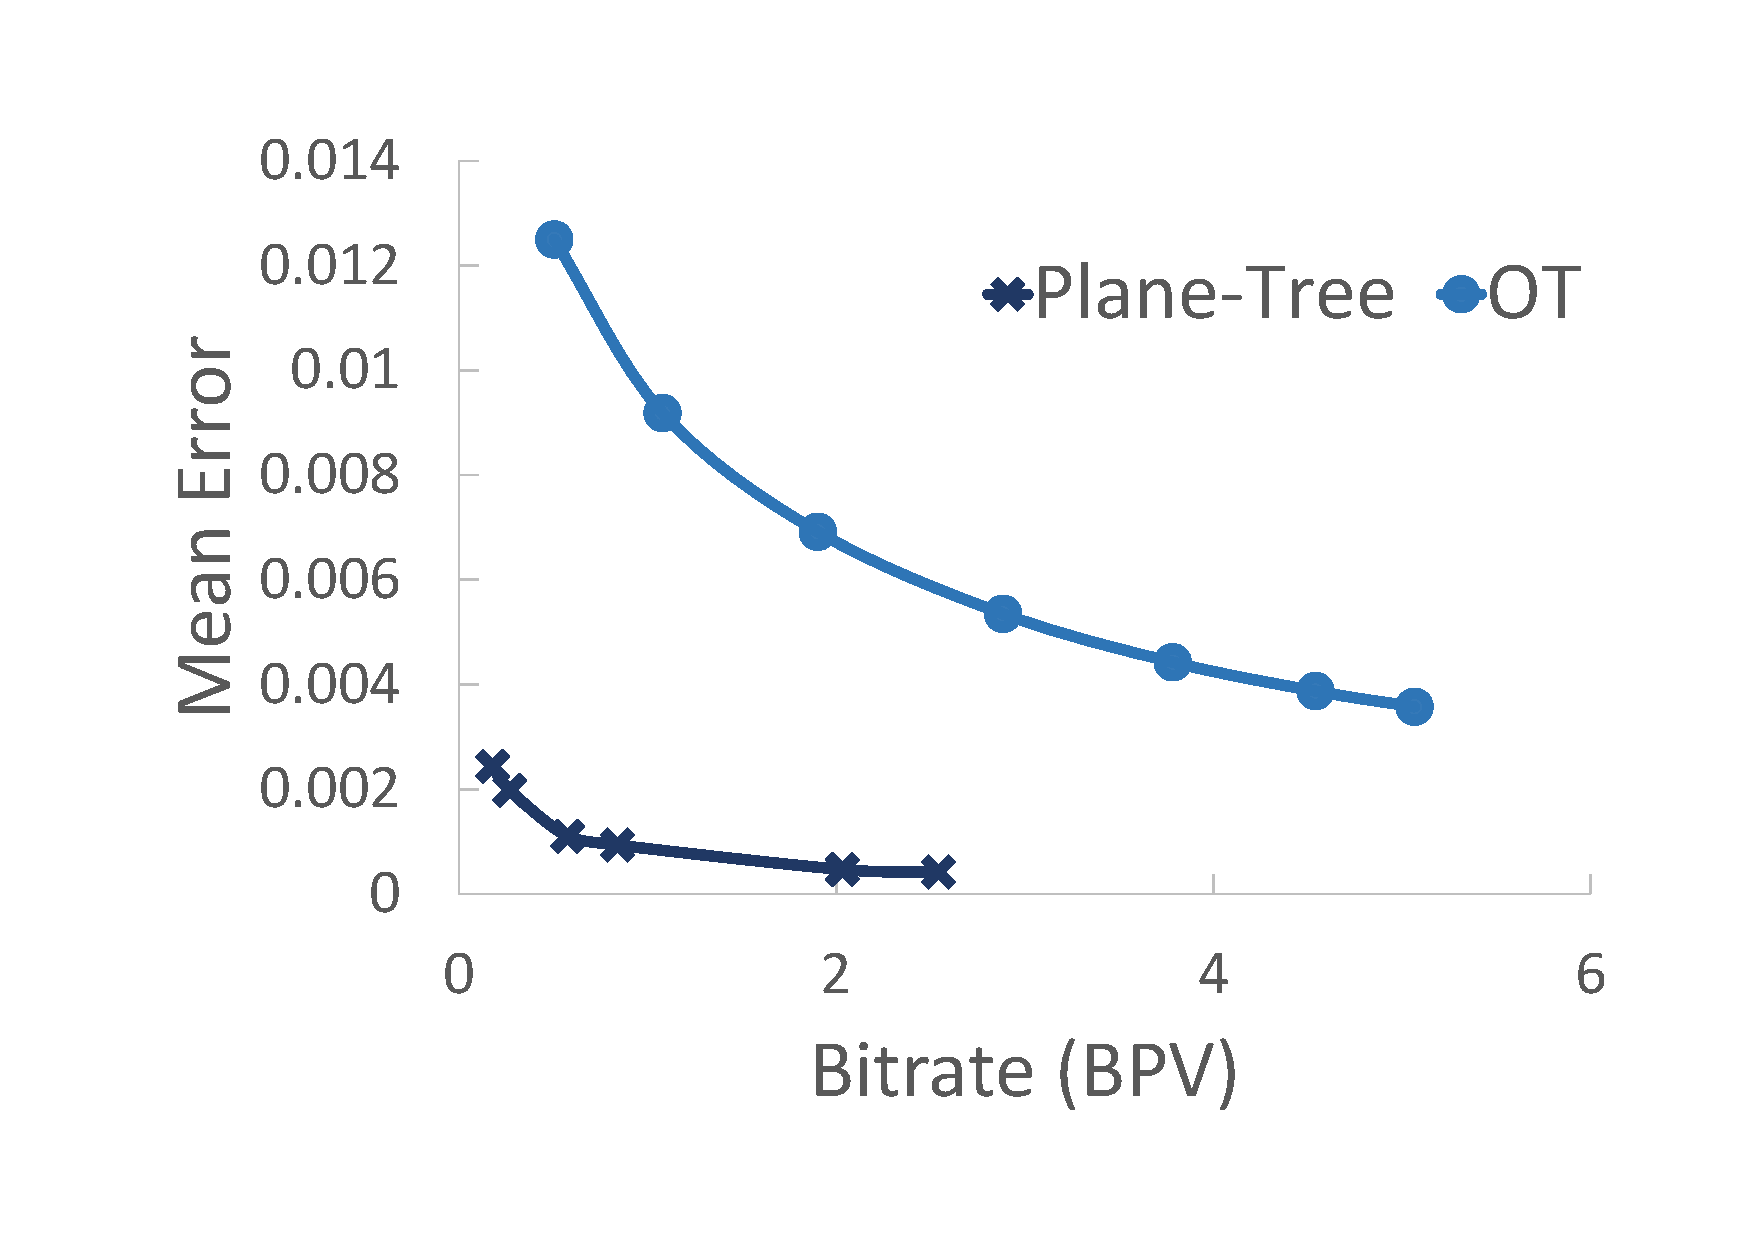
\includegraphics[width=2.5in]{images/results/compression/OTbunny}
                \caption{Bunny Model}
                \label{fig:OG_BUNNY}
        \end{subfigure}%
        \begin{subfigure}[b]{2.8in}
                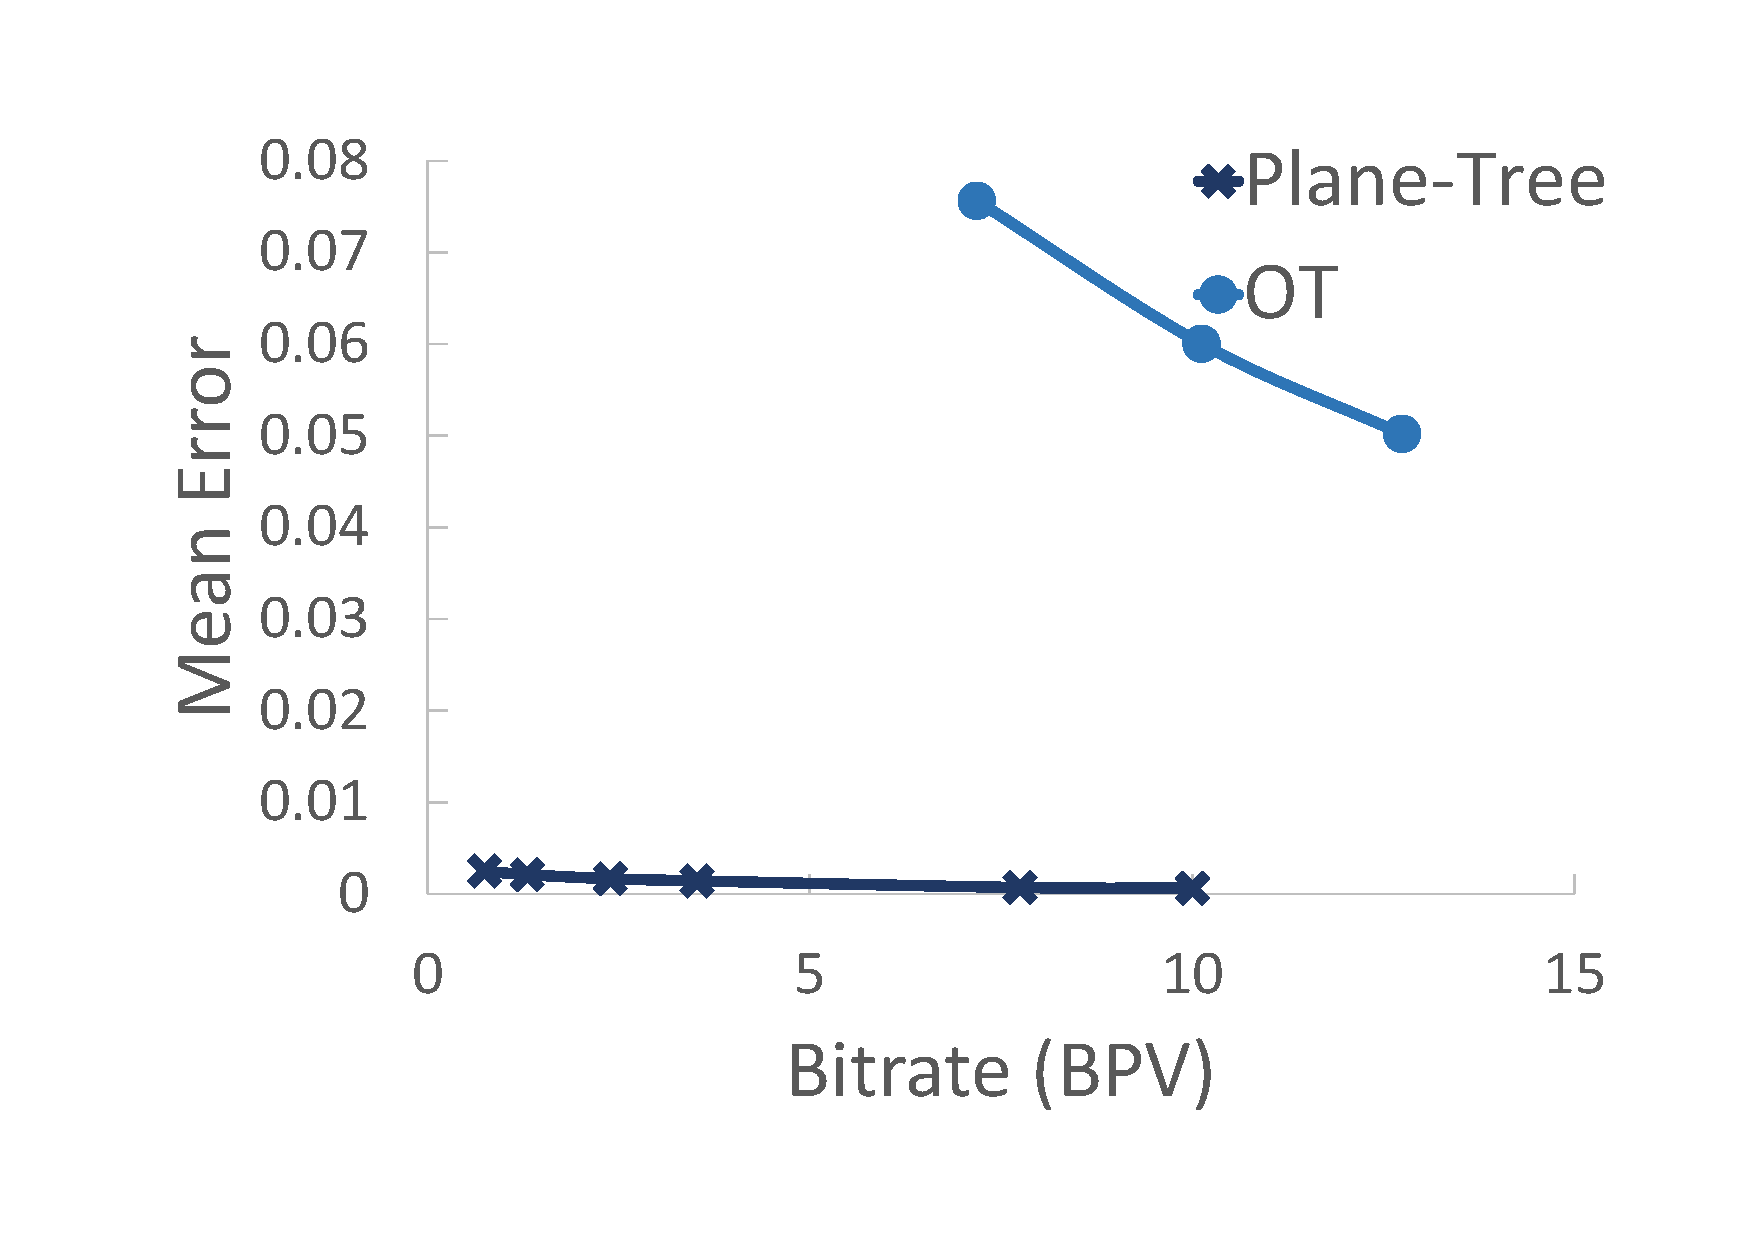
\includegraphics[width=2.5in]{images/results/compression/OTFandisk}
                \caption{Fandisk Model}
                \label{fig:OG_FANDISK}
        \end{subfigure}
        
        \begin{subfigure}[b]{2.8in}
                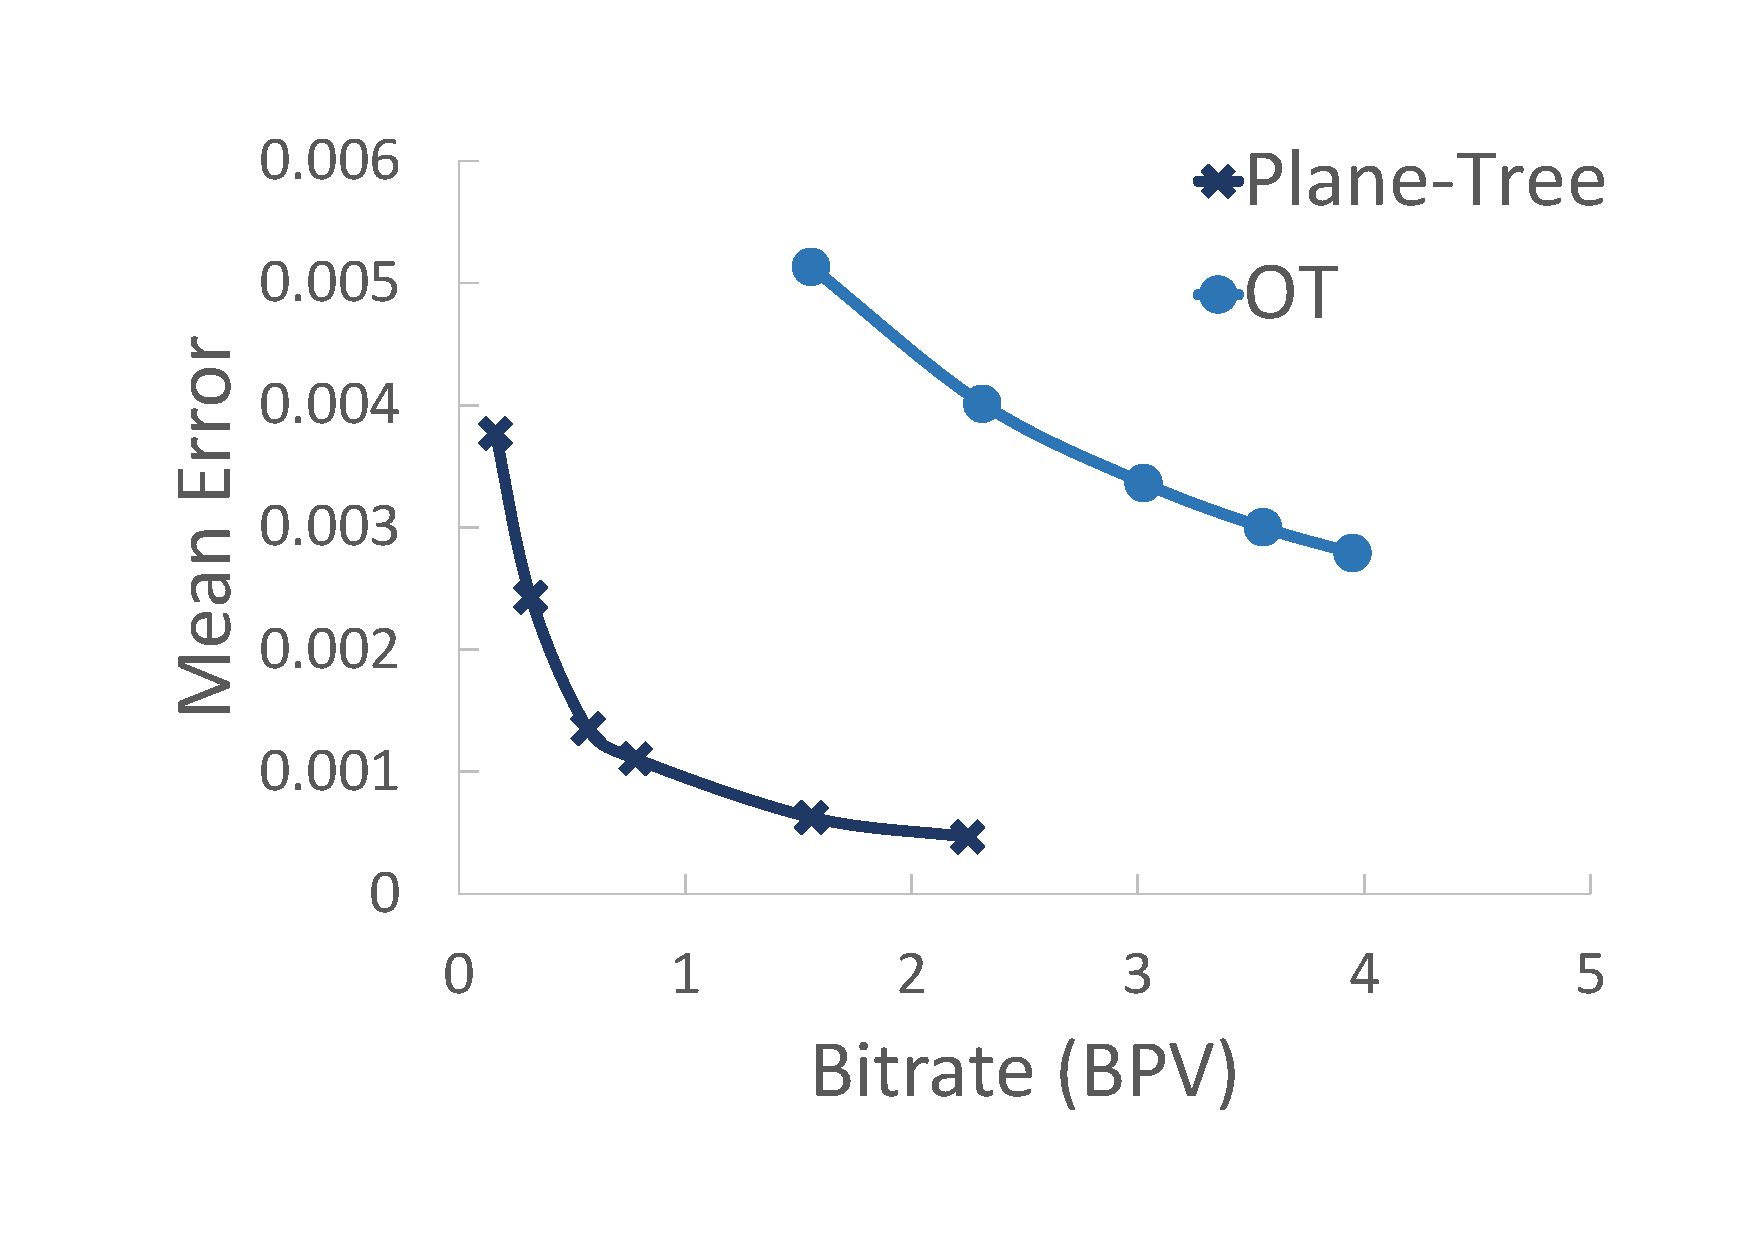
\includegraphics[width=2.5in]{images/results/compression/OTHorse}
                \caption{Horse Model}
                \label{fig:OG_HORSE}
        \end{subfigure}%

       \caption{Rate-distortion graphs comparing the Plane-Tree with the Octree.}
       \label{fig:OTEXPS}
\end{figure}